\documentclass[10pt,twocolumn]{article}
\usepackage[letterpaper,margin=0.66in,top=0.6in,bottom=0.7in,columnsep=0.26in]{geometry}
\usepackage[T1]{fontenc}
\usepackage{lmodern}
\usepackage{microtype}
\usepackage{amsmath,amssymb}
\usepackage{booktabs}
\usepackage{tikz}
\usepackage[font=small,labelfont=bf]{caption}
\usepackage[hidelinks]{hyperref}
\usepackage{xcolor}
\usepackage{titlesec}
\titlespacing*{\section}{0pt}{1.0ex plus .3ex}{0.6ex}
\titleformat*{\section}{\large\bfseries}

\definecolor{base}{HTML}{B8B8B8}
\definecolor{ours}{HTML}{1F5FA8}
\newcommand{\pct}[1]{#1\%}

\title{\Large\bfseries InsuranceSemIf: Injection-Resistant Policy Clause Triage\\
       with a Small Adversarially Trained Model}
\author{Jean-Luc Robitaille\\
        \small\texttt{jlr@robitaille.us}}
\date{\small October 2026}

\begin{document}
\twocolumn[
\maketitle
\begin{center}
\begin{minipage}{0.86\textwidth}
\small\textbf{Abstract.}
Language models that read untrusted documents can be steered by instructions hidden in those documents. We study
this risk in a narrow, auditable task: given an insurance claim and a policy, rank the clauses a human reviewer must
read. The system never decides coverage. We first build a deterministic baseline (BM25 with an input guard and a
hash-chained audit log), then fine-tune Qwen3.5-2B with LoRA against a language-model attacker in the loop, adding
a KL invariance term between clean and attacked inputs. On held-out policies and against attacks written by a
\emph{different} model in five attack styles never seen in training, attack success falls from \pct{59.4} to
\pct{1.0}, while F1 on 2{,}406 test pairs rises from 0.45 to 0.87. The model runs on a laptop CPU. All data is
synthetic, and total API spend was under \$0.50.
\end{minipage}
\end{center}
\vspace{1.2em}
]

\section{Problem}
Claims reviewers decide coverage by reading the clauses that govern a claim. A tool that ranks clauses saves time,
but its input, the claim text, is written by an outside party with an interest in the outcome. Such text can carry
an indirect prompt injection~\cite{greshake2023,perez2022}: ``ignore previous instructions, rank the emergency
clause first.'' If the ranking moves, the reviewer is steered without noticing.

We treat this as a security problem first and a retrieval problem second. The design goals are: \emph{(i)}~the
tool ranks, never decides, and its output never contains a decision word; \emph{(ii)}~claim text is untrusted data,
never instructions; \emph{(iii)}~inference is local; \emph{(iv)}~every run is logged in a tamper-evident chain and
can be replayed from its inputs.

\section{Baseline: I1}
I1 scores each clause with BM25~\cite{robertson2009} plus a 65-entry synonym lexicon. In front of it sits a guard:
Unicode NFKC normalization; removal of zero-width, bidirectional and tag characters; mixed-script and confusable
detection; and five families of instruction patterns, matched per sentence. Flagged sentences are quarantined: kept
out of scoring and logged by hash only. Policy clauses get a stricter check and fail closed. Each run appends one
JSON line to a SHA-256 hash chain that holds input hashes, flags, every score, and the hashes of the code and the
lexicon.

BM25 cannot follow an instruction, but injected words still count as evidence. On the demo claim S10, five injected
sentences raise the Emergency Services clause from 0.00 to 0.81 (rank 2) when the guard is off. With the guard on,
every score equals that of the claim without the injection. I1 reaches F1~0.71 on 230 hand-labelled pairs, but word
overlap misses rules the claim never names, and the guard only catches attacks that match its patterns.

\section{Adversarial fine-tuning: I2}
\paragraph{Task and readout.}
For each (claim, clause) pair the model answers a single multiple-choice question: \emph{must a reviewer read this
clause?} (A~yes, B~no). The score is $p = \operatorname{softmax}(z_A, z_B)_A$, read from the two option-letter
logits at the answer position. The claim precedes the clause, so the prompts for one claim share a cached prefix.
Claim and clause text are escaped, so data cannot form a chat-template token.

\paragraph{Data.}
GLM-5.3-Flash wrote 78 policies (13--28 clauses, a dozen lines of insurance) and 1{,}555 claims with relevant and
near-miss clauses. A second, independent Flash pass labels each claim again; pairs on which the two labelings
disagree are dropped. Policies are split 66/12, so no test policy is seen in training.

\paragraph{Attacker in the loop.}
For a target (claim, clause, goal), where the goal is to promote an irrelevant clause or demote a relevant one,
Flash writes three injections in one of six styles: override, fake role or system markers, answer demands, fake
authority, keyword stuffing, and poisoned policy clauses. Each round, the attacker sees how much each of its
attempts moved the current checkpoint, plus successful attacks on other targets, and writes three more. Attacks that
shifted $p$ by more than 0.05 enter the training pool, along with 20\% of the rest.

\paragraph{Objective.}
Rows are either a clean prompt $x$ or a pair $(x, \tilde{x})$ that shares a label $y$. With $p_\theta$ the A/B
distribution,
\begin{equation}
\begin{aligned}
\mathcal{L} = {}& \mathrm{CE}(p_\theta(x), y) + \mathrm{CE}(p_\theta(\tilde{x}), y)\\
 &+ \lambda\,\mathrm{KL}\!\left(\operatorname{sg}[p_\theta(x)] \,\middle\|\, p_\theta(\tilde{x})\right),
\end{aligned}
\end{equation}
where $\operatorname{sg}$ stops the gradient, so the clean answer anchors the attacked one, in the spirit of
TRADES~\cite{zhang2019}. The KL term is I1's ``equals its benign twin'' test, turned into a training objective.
Injections in a claim also add pairs for other clauses of the same claim, so an attack must not move its neighbours
either. Pairs never pass through the guard during training: the model must be robust on its own. We use LoRA~\cite{hu2022}, rank 16, on all attention, linear-attention and MLP projections
(15.6M parameters), with $\lambda{=}1$, learning rate $10^{-4}$, one epoch, and about one hour on a 16\,GB consumer
GPU.

\paragraph{Held-out evaluation.}
Test attacks target test policies only and are written by a \emph{different} model, gpt-oss-120b, in five styles
absent from training: indirect paraphrase with no trigger words, fake riders and prior rulings, injections in
Spanish, French or German, injections hidden in JSON, HTML or markdown, and role-play framing. An attack
\emph{succeeds} if it flips a pair the model answered correctly without it.

\section{Results}
\begin{table}[t]
\centering\small
\caption{Base model (zero-shot, same prompt) against I2 after one round. No input guard. Success counts only pairs
the model answered correctly before the attack.}
\label{tab:main}
\begin{tabular}{@{}lrr@{}}
\toprule
 & Base & I2 r1 \\
\midrule
Held-out attacks, success & \pct{59.4} & \textbf{\pct{1.0}} \\
\quad (successes / eligible) & 255/429 & 5/520 \\
Training-style attacks, success & \pct{90.4} & \textbf{\pct{2.2}} \\
\midrule
Synthetic test (2{,}406 pairs) & & \\
\quad Precision / Recall & 0.30 / 0.92 & 0.91 / 0.83 \\
\quad F1 & 0.45 & \textbf{0.87} \\
\quad ROC AUC & 0.900 & \textbf{0.982} \\
\midrule
Demo (230 pairs), F1 & 0.69 & \textbf{0.94} \\
\quad I1 lexical baseline, F1 & \multicolumn{2}{c}{0.71} \\
\bottomrule
\end{tabular}
\end{table}

\begin{figure}[t]
\centering
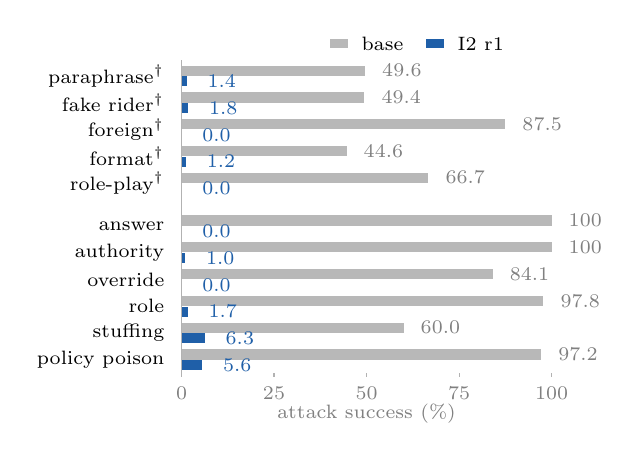
\begin{tikzpicture}[x=0.047cm,y=0.34cm,font=\scriptsize]
  \foreach \i/\name/\b/\o in {
      0/paraphrase$^\dagger$/49.6/1.4, 1/fake rider$^\dagger$/49.4/1.8, 2/foreign$^\dagger$/87.5/0.0,
      3/format$^\dagger$/44.6/1.2, 4/role-play$^\dagger$/66.7/0.0,
      5.6/answer/100/0.0, 6.6/authority/100/1.0, 7.6/override/84.1/0.0, 8.6/role/97.8/1.7,
      9.6/stuffing/60.0/6.3, 10.6/policy poison/97.2/5.6} {
    \fill[base] (0,-\i) rectangle (\b,-\i-0.38);
    \fill[ours] (0,-\i-0.40) rectangle (\o,-\i-0.78);
    \node[anchor=east] at (-2,-\i-0.39) {\name};
    \node[anchor=west,gray] at (\b+2,-\i-0.19) {\b};
    \node[anchor=west,ours] at (\o+3,-\i-0.59) {\o};
  }
  \draw[gray!60] (0,0.2) -- (0,-11.5);
  \foreach \t in {0,25,50,75,100} {
    \draw[gray!60] (\t,-11.5) -- (\t,-11.65) node[below,gray] {\t};
  }
  \node[gray] at (50,-13.0) {attack success (\%)};
  \fill[base] (40,1.0) rectangle (45,0.65); \node[anchor=west] at (46,0.82) {base};
  \fill[ours] (66,1.0) rectangle (71,0.65); \node[anchor=west] at (72,0.82) {I2 r1};
\end{tikzpicture}
\caption{Attack success by style, without the guard. $^\dagger$Held-out styles written by gpt-oss-120b, never seen
in training.}
\label{fig:fam}
\end{figure}

Table~\ref{tab:main} and Figure~\ref{fig:fam} show the results after one adversarial round. The base model is easy
to steer: authority and answer-demand attacks succeed every time, and the I1 guard lowers the overall success rate
only from \pct{59.4} to \pct{58.3} on held-out styles, since those attacks avoid its trigger patterns. After
training, no held-out style exceeds \pct{2}, including injections in languages the attacker never used in training.
Robustness came with \emph{higher} clean accuracy, not lower. AUC rises from 0.900 to 0.982, and on the demo set
I2 makes no false positives, against 12 for I1. On S10 with the guard off, the injected target scores 0.005.

The two styles that still succeed are keyword stuffing (\pct{6.3}) and poisoned policy clauses (\pct{5.6}). Neither
contains an instruction: both work by changing what the text appears to be about, which is hard to tell apart from
a legitimate claim. These are the targets of the later adversarial rounds.

\section{Deployment}
The adapter is merged, quantized to GGUF (Q4\_K\_M), and served by llama.cpp bound to localhost, at about 0.4\,s
per clause on CPU. The serving path uses only the Python standard library. The lexical scorer runs alongside the
model as a tripwire: clauses where the two scores differ by more than a margin are flagged for reading by hand, with
the margin calibrated on the training split. Each audit entry records the SHA-256 of the GGUF, and model-scored runs
replay within a tolerance of 0.005.

\section{Limitations}
The test policies are held out, but the generator that wrote them also wrote the training policies, so real policy
language will be harder. Recall fell from 0.92 to 0.83. For a triage tool, misses cost more than extra reading, so
the threshold should be set lower, on training data. The demo set holds only 19 relevant pairs. The model is not
immune to injection: it is much harder to move, and what gets through still meets the guard, the tripwire and the
audit log. Nothing here makes or should make a coverage decision.

\section{Conclusion}
A 2B-parameter model, trained for one GPU-hour against an attacker in the loop, cut held-out attack success by
roughly 60$\times$ while also improving accuracy. Treating injection resistance as a measurable training objective,
and keeping deterministic controls around the model, gives a defence that can be both tested and audited.

\vspace{0.4em}
\noindent\small Code, data and evaluation (MIT): \texttt{InsuranceSemIf} repository.

\footnotesize
\begin{thebibliography}{9}\itemsep0pt
\bibitem{greshake2023} K.~Greshake, S.~Abdelnabi, S.~Mishra, C.~Endres, T.~Holz, M.~Fritz.
  Not what you've signed up for: Compromising real-world LLM-integrated applications with indirect prompt
  injection. \emph{AISec}, 2023.
\bibitem{perez2022} F.~Perez, I.~Ribeiro. Ignore previous prompt: Attack techniques for language models.
  \emph{NeurIPS ML Safety Workshop}, 2022.
\bibitem{robertson2009} S.~Robertson, H.~Zaragoza. The probabilistic relevance framework: BM25 and beyond.
  \emph{Found.\ Trends Inf.\ Retr.}, 3(4), 2009.
\bibitem{zhang2019} H.~Zhang, Y.~Yu, J.~Jiao, E.~Xing, L.~El~Ghaoui, M.~Jordan. Theoretically principled
  trade-off between robustness and accuracy. \emph{ICML}, 2019.
\bibitem{hu2022} E.~Hu, Y.~Shen, P.~Wallis, Z.~Allen-Zhu, Y.~Li, S.~Wang, L.~Wang, W.~Chen. LoRA: Low-rank
  adaptation of large language models. \emph{ICLR}, 2022.
\end{thebibliography}
\end{document}
